	\documentclass[11pt]{book}
	
	\usepackage{amsfonts,amsthm, bm,amsmath, bbm,amssymb,mathtools}
	\usepackage{fullpage}
	\usepackage{tikz, pgfplots} % added for Lecture 2	
	\usepackage{float}  % added for Lecture 8
	
	\newtheorem{theorem}{Theorem}[chapter]
	\newtheorem{lemma}[theorem]{Lemma}
	
	\theoremstyle{definition}
	\newtheorem{definition}[theorem]{Definition}
	\newtheorem{example}[theorem]{Example}
	\newtheorem{xca}[theorem]{Exercise}
	\newtheorem{corollary}[theorem]{Corollary}  % added for Lecture 5
	\newtheorem{proposition}{Proposition}[section]  % added for Lecture 6
		
	\theoremstyle{remark}
	\newtheorem{remark}[theorem]{Remark}
	
	\numberwithin{section}{chapter}
	\numberwithin{equation}{chapter}
	
	\makeindex
	
	\def\lectureformat{1}
	\usepackage{color}
\usepackage{lipsum}

\ifnum\lectureformat=1
\newcommand{\metadata}[3]
{
	\newpage
	
	\def\lectureID{#1}
	
	\setcounter{chapter}{\lectureID}

%	\draftnotice
	
	\begin{center}
		\bf\large CS229M/STATS214: Machine Learning Theory
	\end{center}
	
	\noindent
	Lecturer: Tengyu Ma   %%% FILL IN LECTURER (if not RS)
	\hfill
	Lecture \# \lectureID              %%% FILL IN LECTURE NUMBER HERE
	\\
	Scribe: #2                  %%% FILL IN YOUR NAME HERE
	\hfill
	#3           %%% FILL IN LECTURE DATE HERE
	
	\noindent
	\rule{\textwidth}{1pt}
	
	\medskip
}
\else 
\newcommand{\metadata}[3]{}
\fi

\newcommand*\circled[1]{\tikz[baseline=(char.base)]{
	\node[shape=circle,draw,inner sep=2pt] (char) {#1};}}

\DeclareMathOperator*{\Exp}{\mathbb{E}}
\DeclareMathOperator*{\argmin}{\textup{argmin}}
\DeclareMathOperator*{\argmax}{\textup{argmax}}

\newcommand{\Cov}{\operatorname{Cov}}
\newcommand{\KL}{\operatorname{KL}}
\newcommand{\margin}{\text{margin}}
\newcommand{\poly}{\operatorname{poly}}
\newcommand{\sd}{\operatorname{sd}}
\newcommand{\sgn}{\text{sgn}}
\newcommand{\tr}{\operatorname{tr}}
\newcommand{\Var}{\operatorname{Var}}

\newcommand{\err}{\ell_{\textup{0-1}}}
\newcommand{\Err}{L_{\textup{0-1}}}
\newcommand{\thetaerm}{\theta_{\textup{ERM}}}
\newcommand{\hatL}{\widehat{L}}
\newcommand{\tilO}{\widetilde{O}}
\newcommand{\iid}{\overset{\textup{iid}}{\sim}}
\newcommand\defeq{\stackrel{\mathclap{\tiny \mbox{$\Delta$}}}{=}}

\newcommand{\norm}[1]{\|#1\|}
\newcommand{\Norm}[1]{\left\|#1\right\|}
\renewcommand{\l}{\left}
\renewcommand{\r}{\right}
\newcommand{\rbr}[1]{\left(#1\right)}
\newcommand{\sbr}[1]{\left[#1\right]}
\newcommand{\cbr}[1]{\left\{#1\right\}}
\newcommand{\abs}[1]{\left\lvert#1\right\rvert}
\newcommand{\inprod}[1]{\left\langle#1\right\rangle}

\newcommand{\al}[1]{
	\begin{align}
	#1
	\end{align}
}

\renewcommand{\sp}[1]{^{(#1)}}

\newcommand{\cA}{\mathcal A}
\newcommand{\cB}{\mathcal B}
\newcommand{\cC}{\mathcal C}
\newcommand{\cD}{\mathcal D}
\newcommand{\cE}{\mathcal E}
\newcommand{\cF}{\mathcal F}
\newcommand{\cG}{\mathcal G}
\newcommand{\cH}{\mathcal H}
\newcommand{\cI}{\mathcal I}
\newcommand{\cJ}{\mathcal J}
\newcommand{\cK}{\mathcal K}
\newcommand{\cL}{\mathcal L}
\newcommand{\cM}{\mathcal M}
\newcommand{\cN}{\mathcal N}
\newcommand{\cO}{\mathcal O}
\newcommand{\cP}{\mathcal P}
\newcommand{\cQ}{\mathcal Q}
\newcommand{\cR}{\mathcal R}
\newcommand{\cS}{\mathcal S}
\newcommand{\cT}{\mathcal T}
\newcommand{\cU}{\mathcal U}
\newcommand{\cV}{\mathcal V}
\newcommand{\cW}{\mathcal W}
\newcommand{\cX}{\mathcal X}
\newcommand{\cY}{\mathcal Y}
\newcommand{\cZ}{\mathcal Z}

\newcommand{\bbB}{\mathbb B}
\newcommand{\bbS}{\mathbb S}
\newcommand{\bbR}{\mathbb R}
\newcommand{\bbZ}{\mathbb Z}
\newcommand{\bbI}{\mathbb I}
\newcommand{\bbQ}{\mathbb Q}
\newcommand{\bbP}{\mathbb P}
\newcommand{\bbE}{\mathbb E}
\newcommand{\bbN}{\mathbb N}

\newcommand{\E}{\mathbb{E}}
\newcommand{\N}{\mathbb{N}}
\newcommand{\R}{\bbR}
\newcommand{\Z}{\mathbb{Z}}


% for course staff to edit or comment
\def\shownotes{1}  %set 1 to show author notes
\ifnum\shownotes=1
\newcommand{\authnote}[2]{[#1: #2]}
\else
\newcommand{\authnote}[2]{}
\fi
\newcommand{\tnote}[1]{{\color{blue}\authnote{TM}{#1}}}

% for long term comments 
\def\shownotes{0}  %set 1 to show author notes
\ifnum\shownotes=1
\newcommand{\authnotelong}[2]{[#1: #2]}
\else
\newcommand{\authnotelong}[2]{}
\fi
\newcommand{\tnotelong}[1]{{\color{blue}\authnotelong{TM}{#1}}}
	\begin{document}
	
	\frontmatter
	
	\mainmatter
	\let\sec\section
	\let\subsec\subsection
	
	\newcommand{\secwarning}[1]{
		{	
			\color{red}
			$\backslash$section and $\backslash$subsection are disallowed, please use 	$\backslash$sec and $\backslash$subsec instead
		}
	}
	\let\section\secwarning
	\let\subsection\secwarning
	
	
	\newcommand{\draftnotice}{\vbox to 0.25in{\noindent
			\raisebox{0.6in}[0in][0in]{\makebox[\textwidth][r]{\it
					DRAFT --- a final version will be posted shortly}}}
		\vspace{-.25in}\vspace{-\baselineskip}
	}
	
	%\section{}
	% reset section counter
\setcounter{section}{0}

%\metadata{lecture ID}{Your names}{date}
\metadata{10}{Kevin Han and Han Wu}{Feb 17th, 2021}

\sec{Review and overview}

Last lecture, we outlined conceptual topics in deep learning theory and how the situation was different from classical machine learning theory. In particular, we described \textit{approximation theory}, \textit{statistical generalization} and \textit{optimization}. In this lecture, we will focus on optimization theory in deep learning. We will introduce some basics about optimization, discuss how we can make the notion ``all local minimums are global minimums'' rigorous, and walk through two examples where this is the case.

\sec{Optimization landscape}

The big question that we have in mind is the following: many existing optimizers are designed for optimizing convex functions. \textbf{Why do they still work well for non-convex functions?} We note that it is not true that these optimizers always work well with non-convex functions: there are still some very hard cases that give trouble (e.g. very deep feed-forward networks are still hard to fit because of issues like vanishing and exploding gradients). One possible reason is that the non-convex functions that we are minimizing in deep learning usually have some nice properties: see Figure \ref{lec10:fig:optimization} for an illustration.

\begin{figure}[H]
    \centering
    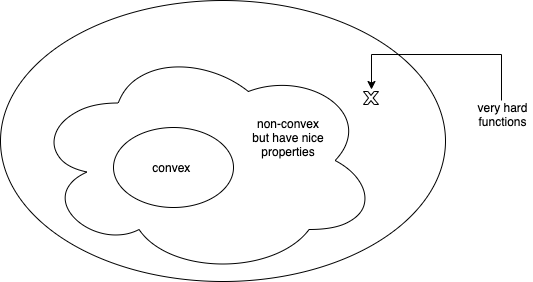
\includegraphics[scale = 0.5]{figures/landscape.png}
    \caption{Classification of different functions for optimization. The functions we optimize in deep learning seem to fall mostly within the middle cloud.}
    \label{lec10:fig:optimization}
\end{figure}

\begin{figure}[H]
    \centering
    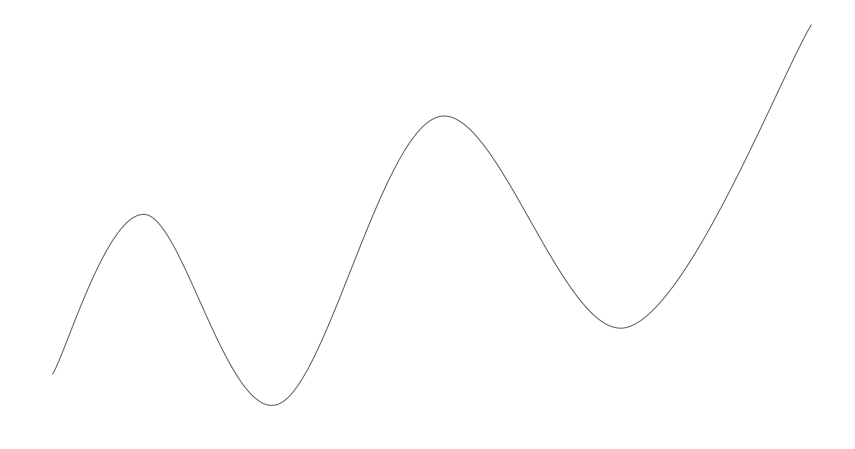
\includegraphics[scale = 0.3]{figures/smooth_func.png}
    \caption{Illustration of a general non-convex function. A useful plot to keep in mind when thinking about non-convex functions. \tnote{I think this plot was to show that you can converge to a bad local minimum. I did draw some arrows in it to show you can converge to a bad local minimum. The problem is that this is not the right picture to keep in mind for high-dimensional nonconvex functions}}
    \label{lec10:fig:smooth_func}
\end{figure}
Before diving into details, we first highlight some observations that will be important to keep in mind when discussing optimization in deep learning. Suppose $g(\theta)$ is the loss function. Recall that the \textit{gradient descent (GD)} algorithm would do the following:
\begin{enumerate}
    \item $\theta_0$ := initialization
    \item $\theta_{t + 1} = \theta_t - \eta\nabla g(\theta_t)$, where $\eta$ is the step size.
\end{enumerate}
Here are some observations to :
\begin{enumerate}
    \item[] \textit{Observation 1}: Gradient descent cannot always find the global minimum.
    \item[] \textit{Observation 2}: Finding the global minimum of general non-convex functions is NP-hard.
    \item[] \textit{Observation 3}: Gradient descent can find the global minimum for convex functions.
    \item[] \textit{Observation 4}: The objective function in deep learning is non-convex.
    \item[] \textit{Observation 5}: Gradient descent/stochastic gradient descent \tnote{+typically} finds an approximate global minimum of loss function in deep learning.
\end{enumerate}

These observations motivate the following two-step plan:

\begin{enumerate}
    \item Identify a large set of functions that stochastic gradient descent/gradient descent can solve.
    \item Prove that some of the loss functions in machine learning problems belong to this set. (Most of the effort will be spent here.)
\end{enumerate}
\textbf{Basic idea:} Gradient descent can find local minimum $+$ all local minimums of $f$ are also global $\Rightarrow$ Gradient descent can find global minimums\tnote{minima; check other places}.

\sec{Convergence to local minimum\tnote{minima}}
Let $f$ be a twice-differentiable function. We start with the following definition:
\begin{definition} [Local minimum of a function]
We say that $x$ is a \textit{local minimum} of a function $f$ if there exists an open neighborhood $N$ around $x$ such that in $N$, the function values are at least $f(x)$.
\end{definition}

Note that if $x$ is a local minimum of $f$, then $\nabla f(x) = 0$ and $\nabla^2 f(x) \succeq 0$. However, as the next example shows, the reverse is not true. When $\nabla f(x) = 0$ and $\nabla^2 f(x)$ vanishes in some direction (i.e. merely positive semi-definite instead of being strictly positive definite), higher-order derivatives start to matter.

\begin{example}
\label{lec10:ex:counterexample}
Consider the function $f(x_1, x_2) = x_1^2 + x_2^3$. $(x_1, x_2) = (0, 0)$ satisfies $\nabla f(x) = 0$ and $\nabla^2 f(x)|_{(x_1, x_2) = (0, 0)} = \begin{bmatrix} 2 & 0 \\
0 & 0\end{bmatrix} \succeq 0$. However, if we move in the negative direction of $x_2$, we can decrease the function value. Hence, this example shows why $\nabla f(x) = 0$ and $\nabla^2 f(x) \succeq 0$ does not imply that $x$ is a local minimum.
\end{example}

It is generally not easy to verify if a point is a local minimum. In fact, we have the following theorem regarding the computational tractability:
\begin{theorem}
\label{lec10:thm:np_hard}
Verifying if $x$ is a local minimum of $f$ is NP-hard. \tnote{Citation} Moreover, finding a local minimum is NP-hard.
\end{theorem}

\subsec{Strict-saddle condition}
Theorem~\ref{lec10:thm:np_hard} forces us to consider more specific types of functions to be able to obtain computational tractability. To this end, we define the following \textit{strict-saddle condition}:

\begin{definition} [Strict-saddle condition (\cite{lee2016}; \tnote{should only cite the first one because the condition in the second one is different}\cite{ge2015})]
For positive $\alpha, \beta, \gamma$, we say that $f: \R^d \mapsto \R$ is \textit{$(\alpha, \beta, \gamma)$-strict-saddle} if every $x \in \bbR^d$ satisfies one of the following:
\begin{enumerate}
    \item $\|\nabla f(x)\|_2 \geq \alpha$.
    \item $\lambda_{\min}(\nabla^2 f(x)) \leq -\beta$.
    \item $x$ is $\gamma$-close to a local minimum $x^*$ in Euclidean distance, i.e. $\|x - x^*\|_2 \leq \gamma$.
\end{enumerate}
\end{definition}

Intuitively speaking, this definition is saying if a point has zero gradient and positive semi-definite Hessian, it must be close to a local minimum, i.e. there is no pathological case like Example \ref{lec10:ex:counterexample}.

We have the following theorem for functions that satisfy strict-saddle condition:

\begin{theorem} [Informally stated]
If $f$ is $(\alpha, \beta, \gamma)$-strict-saddle for some positive $\alpha, \beta, \gamma$, then many optimizers (e.g. gradient descent, stochastic gradient descent, cubic regularization) can converge to a local minimum with $\epsilon$-error in Euclidean distance in time $poly \left(d, \frac{1}{\alpha}, \frac{1}{\beta}, \frac{1}{\gamma}, \frac{1}{\epsilon}\right)$.
\end{theorem}

Therefore, if all local minimums are global minimums and the function satisfies the strict-saddle condition, then optimizers can converge to a global minimum with $\epsilon$-error in polynomial time. (See Figure \ref{lec10:fig:strict-saddle} for an example of a function whose local minimums are all global minimums.) The next theorem expresses this concretely by being explicit about the strict-saddle condition:

\begin{theorem}
Suppose $f$ is a function that satisfies the following condition: $\exists  \ \epsilon_0, \tau_0, c > 0$ such that if $x \in \bbR^d$ satisfies $\|\nabla f(x)\|_2 \leq \epsilon < \epsilon_0$ and $\nabla^2 f(x) \succeq -\tau_0I$, then $x$ is $\epsilon^c$-close to a global minimum of $f$. Then many optimizers can converge to a global minimum of $f$ up to $\delta$-error in Euclidean distance in time $poly\left(\frac{1}{\delta}, \frac{1}{\tau_0}, d \right)$.
\end{theorem}

\begin{figure}[H]
    \centering
    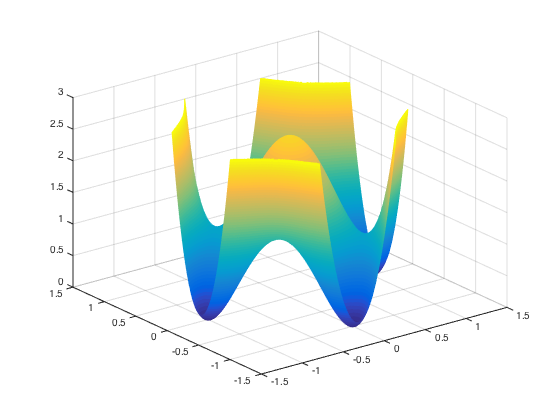
\includegraphics[scale = 0.5]{figures/localmin.png}
    \caption{A two-dimensional function with the property that all local minimums are global minimums. It also satisfies the strict-saddle condition because all the saddle points have a strictly negative curvature in some direction.}
    \label{lec10:fig:strict-saddle}
\end{figure}

\sec{Two examples where local minimums are global minimums\tnote{grammar; many other places}}
So far, we have focused on general results. Next, we give two concrete examples that satisfies all local minimums are global minimums:(i) principal components analysis (PCA)/matrix factorization/linearized neural nets, and (ii) matrix completion.

\subsec{Principal components analysis (PCA)}
Let matrix $M \in \bbR^{d \times d}$ be symmetric and positive semi-definite. Consider the problem of finding the best rank-1 approximation of the matrix $M$. The objective function here is non-convex:
\begin{equation}
    \min_{x \in \bbR^d}g(x) \triangleq \frac{1}{2}\|M - xx^T\|_F^2.
\end{equation}

\begin{theorem}
All local minimums of $g$ are global minimums (even though $g$ is non-convex).
\end{theorem}

\begin{remark}
For $d = 1$, $g(x) = (m - x^2)^2$ for some constant $m$. Figure~\ref{lec10:fig:pca_objective} below shows such an example. We can see that all local minimums are indeed global minimums.
\end{remark}

\begin{figure}[H]
    \centering
    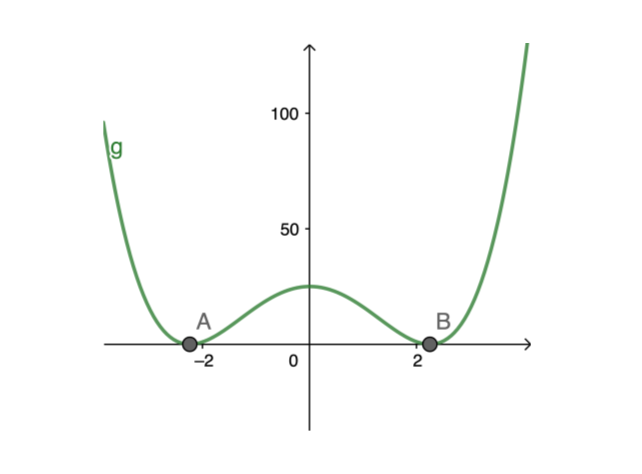
\includegraphics[scale = 0.4]{figures/pca.png}
    \caption{Objective function for principal components analysis (PCA) when $d = 1$.}
    \label{lec10:fig:pca_objective}
\end{figure}

\begin{proof}

\textit{Step 1: Show that all stationary points must be eigenvectors.} From HW0, we know that $\nabla g(x) = -(M - xx^T)x$, hence
\begin{equation}\label{lec10:eqn:pca-firstorder}
\nabla g(x) = 0 \implies Mx = \|x\|_2^2\cdot x,
\end{equation}
which implies that $x$ is an eigenvector of $M$ with eigenvalue $\|x\|_2^2$. From the Eckart–Young–Mirsky theorem we know the global minimum (i.e. the best rank-1 approximation) is the eigenvector with the largest eigenvalue.

\textit{Step 2: Show that all local minimums must be eigenvectors of the largest eigenvalue.} We use the second order condition for this. For $x$ to be a local minimum we need $\nabla^2g(x) \succeq 0$, which means for any $v \in  \bbR^d$, 
\begin{equation}
\langle v, \nabla^2g(x) v \rangle \geq 0.
\end{equation}
To compute $\langle v, \nabla^2g(x) v \rangle$, we use the following trick: expand $g(x + v)$ into $g(x) + \text{linear term in } v + \text{quadratic term in } v$, then the quadratic term will be $\langle v, \nabla^2g(x) v \rangle$ (see HW0 Problem 2d for an example). Using this trick, we get 
\tnote{could the scribe notes taker fill in this derivation?}
\begin{equation}
\langle v, \nabla^2g(x) v \rangle = 2\langle x, v \rangle^2 - v^TMv + \|x\|_2^2\|v\|_2^2. 
\end{equation}
Picking $v = v_1$, the unit eigenvector with the largest eigenvalue (denoted $\lambda_1$), for $x$ to be a local minimum it must satisfy 
\begin{equation}
\langle v_1, \nabla^2g(x) v_1 \rangle = 2\langle x, v_1 \rangle^2 - v_1^TMv_1 + \|x\|_2^2 \geq 0.
\end{equation}

Note that by \eqref{lec10:eqn:pca-firstorder}, all our candidates for local minimums are eigenvectors of $M$ so naturally we have two cases:
\begin{itemize}
\item \textit{Case 1: $x$ has eigenvalue $\lambda_1$}. Then x is the global minimum (by the Eckart–Young–Mirsky theorem).
\item \textit{Case 2: $x$ has eigenvalue $\lambda < \lambda_1$}. Then we know $x$ and $v_1$ are orthogonal (eigenvectors with different eigenvalues are always orthogonal), hence 
\begin{equation}
2\langle x, v_1 \rangle^2 - v_1^TMv_1 + \|x\|_2^2 = 0  -\lambda_1 + \lambda \geq 0,
\end{equation}
which implies $\lambda \geq \lambda_1$, a contradiction. 
\end{itemize}

In summary, if $x$ is a stationary point and $x$ is not a global minimum, then moving in the direction of $v_1$ would lead to second-order improvement and $x$ cannot be a local minimum. 
\end{proof}

\subsec{Matrix Completion \cite{ge2016}}
We consider rank-1 matrix completion for simplicity. Let $M = zz^T$ be a rank-1 symmetric and positive semi-definite matrix for some $z\in \bbR^d$. Given random entries of $M$, our goal is to recover the rest of entries. Formally, we have the following definitions:

\begin{definition}
Suppose $M\in \bbR^{d\times d}$ and $\Omega \subseteq [d] \times [d]$, we define $P_{\Omega}(M)$ to be the matrix obtained by zeroing out every entry outside $\Omega$. 
\end{definition}

\begin{definition}[Matrix Completion]
Suppose $M\in \bbR^{d\times d}$ and every entry of $M$ is included in $\Omega$ with probability $p$. The \textit{matrix completion task} is to recover $M$ (with respect to some loss functions) given the observation $P_{\Omega}(M)$.
\end{definition}

A nice real world example of matrix completion is when we have a matrix describing the user ratings for each item. We only observe a small portion of the entries as each customer only buys a small subset of the items. A good matrix completion algorithm is indispensable for a recommendation engine. 

\begin{remark}
We need $d$ parameters to describe a rank-1 matrix $M$ and the number of observations is roughly $pd^2$. Thus, for identifiability we need to work in the regime where $pd^2 > d$, i.e. $p \gg \frac{1}{d}$. 
\end{remark}

We define our non-convex loss functions to be 
\begin{align}
    \min_{x \in \bbR^d}g(x) & \triangleq \frac{1}{2}\sum_{(i,j)\in \Omega}(M_{ij}-x_ix_j)^2 \\
     & = \frac{1}{2}\|P_{\Omega}(M-xx^T)\|_F^2.
\end{align}

To really solve our problem we need some regularity condition on the ground truth vector $z$ (recall $M = zz^T$). \textit{Incoherence} is one such condition:
\begin{definition}[Incoherence]
Without loss of generality, assume the ground truth vector $z\in\bbR^d$ satisfies $\|z\|_2 = 1$. $z$ satisfies the \textit{incoherence condition} if $\|z\|_{\infty} \leq \frac{\mu}{\sqrt{d}}$, where $\mu$ is considered to be a constant or log in dimension $d$. 
\end{definition}

\begin{remark}
A nice counterexample to think about why such condition is necessary is when $z = \mathbf{e_1}$ and $M = \mathbf{e_1}\mathbf{e_1}^T$. \tnote{could we avoid using bold font for symbols?} All entries of $M$ are 0 except for a 1 in the top-left corner. There is no way to recover $M$ without observing the top-left corner.
\end{remark}

We conclude with a theorem which we will prove next lecture:
\begin{theorem}
Suppose $p = \frac{poly(\mu, \log d)}{d\epsilon^2}$ for some sufficient small constant $\epsilon$ and assume $z$ is incoherent. Then all local minimums of $f$ are $O(\sqrt{\epsilon})$-close to either $z$ or $-z$ (i.e. the global minimums), and we also have the strict saddle condition.
\end{theorem}


	
	%    Include main chapters here.
	%\include{}
	\appendix
	%    Include appendix "chapters" here.
	
	
	%\backmatter
	%    Bibliography styles amsplain or harvard are also acceptable.
	\bibliographystyle{amsalpha}
	\bibliography{bibliography}
	%    See note above about multiple indexes.
%	\printindex
	
	\end{document}
	
	%-----------------------------------------------------------------------
	% End of amsbook-template.tex
	%-----------------------------------------------------------------------
